\documentclass[a4paper, 11pt]{scrreprt}

\usepackage[a4paper, top=2cm]{geometry} % Use A4 paper size
\usepackage{color} % Required for color customization
\usepackage[english]{babel}
\usepackage[T1]{fontenc}
\usepackage{url}
\usepackage{cite}
\usepackage{amsmath,amssymb,amsfonts}
\usepackage{algorithmic}
\usepackage{graphicx}
\usepackage{subfig}
\usepackage{float}
\usepackage{textcomp}
\usepackage{xcolor}
\usepackage{tikz}
\usepackage[section]{placeins}
\usepackage[justification=centering]{caption}
\usepackage{calc}
\usepackage[nomessages]{fp}
\usepackage{parskip}    
\usepackage{bold-extra} % that's new
\usepackage{setspace}
\usepackage{fancyhdr}
\usepackage{titlesec}
\usepackage{lmodern}

\usepackage[T1]{fontenc} % optional
\usepackage{lmodern}

\usepackage[utf8]{inputenc}
\usepackage[cmintegrals]{newtxmath}
\usepackage{bm} % optional

\usepackage{listings}
\usepackage{listings-ext}

\usepackage{glossaries}
\usetikzlibrary{positioning}% for positioning of nodes
\usetikzlibrary{shapes, arrows, shapes.geometric, shadows,positioning}

\usepackage[
    pdftitle={Failsafe ECU through Dynamic Partial Reconfiguration in FPGAs},
    pdfauthor={Constantin Schieber, Rupert Schorn, Andreas Hirtenlehner, Peter Schober},
    pdfsubject={Documentation},
    colorlinks=true,
    hyperindex=true,
    plainpages=false,
    pdfpagelabels=true,
    bookmarksopen=false,
    linktocpage=true
]{hyperref}

\DeclareUnicodeCharacter{2011}{-}

\makeglossaries
\loadglsentries{glsEntries}

%\usetikzlibrary{external}
%\tikzexternalize % activate!

\newlength{\smallColumnWidth}
\setlength{\smallColumnWidth}{\columnwidth-2cm}%

\hypersetup{colorlinks,linkcolor=[rgb]{0,0.4,0.6},filecolor=red,urlcolor=[rgb]{0,0.4,0.6},citecolor=[rgb]{0,0.4,0.6}}

% sets the pagelayout
%\setlength{\oddsidemargin}{4mm}
%\setlength{\evensidemargin}{-6mm}
%\setlength{\textwidth}{162mm} 
%\setlength{\textheight}{230mm}
%\setlength{\topmargin}{-5mm}

\pagestyle{fancy}

\fancyhf{}
\renewcommand{\chaptermark}[1]{\markboth{#1}{}}
\fancyhead[RO]{\rightmark}
\fancyhead[LE]{\leftmark}
\fancyfoot[C]{\thepage}

% no headers on chapter pages
\fancypagestyle{plain}{%
    \fancyhf{} % clear all header and footer fields
    \fancyfoot[C]{\thepage} % except the center
    \renewcommand{\headrulewidth}{0pt}
    \renewcommand{\footrulewidth}{0pt}
}

% no numbers on part pages
\renewcommand*{\partpagestyle}{empty}

% sonst können sehr große Abstände zwischen Überschriften und Zeilen vorkommen
\raggedbottom

% 1.5 Facher Zeilenabstand
\onehalfspacing

% no numbers on part pages in TOC
%\makeatletter
%\let\partbackup\l@part
%\renewcommand*\l@part[2]{\partbackup{#1}{}}
%\makeatother

% vertical space under subsubsection
%\titlespacing{\subsubsection}{0pt}{\parskip}{-\parskip}

%vertical destance between paragraphs
\setlength{\parskip}{0.3\baselineskip}

%vertical distance between bib items
%\setlength\bibitemsep{0.5\baselineskip}




\begin{document}

\pagestyle{plain}
\begin{titlepage}

\begin{doublespace} 
\begin{center}
    \vspace*{35mm}
    {\LARGE\textbf{Dynamic Partial Reconfiguration for Fault-Tolerance in automotive ECUs}}\\
    \vspace*{5mm}
    {\large 384.157 Labor SoC Design, WS 2018}
    \vspace*{20mm}
\end{center}
\end{doublespace}

\begin{figure}[H]
    \begin{center}
    	\includegraphics[scale=0.3]{./figures/TU_logo.pdf}
	    \label{fig:logo}
    \end{center}
\end{figure}

\vfill

\begin{tabular}{ll} 
    Constantin Schieber & 1228774\\[1mm]
    Rupert Schorn & 1325700\\[1mm]
    Andreas Hirtenlehner & 1327273\\[1mm]
    Peter Schober & 1355178\\[5mm]
    \multicolumn{2}{l}{\today} 
\end{tabular}

\end{titlepage}

\cleardoublepage
\pagenumbering{Roman} 

{
  \tableofcontents
  \newpage
  %\addcontentsline{toc}{section}{Kurzfassung}
\null\vfill

% Deutsche Kurzfassung
%\begin{center}
%\textbf{Kurzfassung}
%\vspace*{5mm}
%\end{center}
%-- KURZFASSUNG --
%\vspace*{20mm}

% Abstract in english
\begin{center}
\textbf{Abstract}
\vspace*{5mm}
\end{center}
In this lab, fail-safe mechanisms for \glspl{ECU} are explored on the basis of \gls{PR} in \glspl{FPGA}.
The introduced design contains typical characteristics of an automotive system.
Communication between the different sub-systems is realized by a specific link (including protocol) and connects the \gls{FPGA} to the \glspl{ECU} that handle operations during normal conditions. 
\glspl{ECU} are monitored by a bus monitor in the \gls{FPGA} for nominal operation characteristics and can be replaced by the instantiation of the very same \gls{ECU} within the \gls{FPGA} in case of failure.

\par\vfill\vfill
\newpage

  \cleardoublepage
}

\pagenumbering{arabic}

\section{Introduction}
\begin{figure}[t]
    \centering
    \includegraphics[width=\textwidth]{figures/pr_blockDesign.pdf}
    \caption{Block Diagram of the partial reconfiguration functionality}\label{fig:prBlockDesign}
\end{figure}

Brief overview, problem statement and final outcome.

\subsection{Required Tools and packages}

\begin{itemize}
    \item Vivado 2018.3
    \item Vivado 2018.2
    \item uVision 5 (Windows only)
    \item ARM Keil (Windows only)
    \item ARM Cortex M1 IP for Vivado
\end{itemize}

\chapter{Cortex M1 on Xilinx}

Description of the setup of the Cortex M1 core. \cite{arm_arm_2018} \cite{arm_cortex-m1_nodate}

\section{Usage of Cortex M1 in Vivado}

Only global implementation / synthesis runs are permitted to obtain a working bitstream.
If OOC (Out of Context) runs are used, everything except for the Cortex M1 will work fine. 
The Cortex M1 will enter a hard-fault state which does not allow recovery. 
This is indicated by a high bit on the \textit{Lockup} port of the processor.

Also trivial, follow tutorial that is provided on ARM Website and adapt to own needs.

\subsection{Code via Memory Initialization File}

To update the Memory Initialization File for a core, a new package with the updated \textit{bram\_a7.hex} file in the corresponding core (\textit{/cores/cm1\_*/m1\_for\_arty\_a7.srcs/\\sources\_1/imports/m1\_for\_arty\_a7/m1\_for\_arty\_a7/} \cite{fpga_design}) has to be generated and the \gls{IP} in the block design has to be updated.

\section{How to mbed OS}
To achieve a common code base for the application code, Mbed OS, a \gls{RTOS} from ARM, was used (Fig \ref{fig:mbed}). 
Since there is no support for the Xilinx Cortex M1 core, the \gls{BSP} provided by Xilinx was ported to Mbed OS \cite{mbed_port}. 
The port includes the \gls{RTOS} kernel and the GPIO and UART modules. 
The firmware for our \gls{FPGA} design \cite{fpga_design} can be found on GitHub \cite{firmware}. 
For using Mbed OS with a new design, the \gls{BSP} has to be exported from the Vivado SDK and copied to \textit{/mbed-os/targets/TARGET\_Xilinx/TARGET\_XC7Z020/device/standalone\_bsp/} in \cite{firmware}.

\begin{figure}[ht]
    \centering
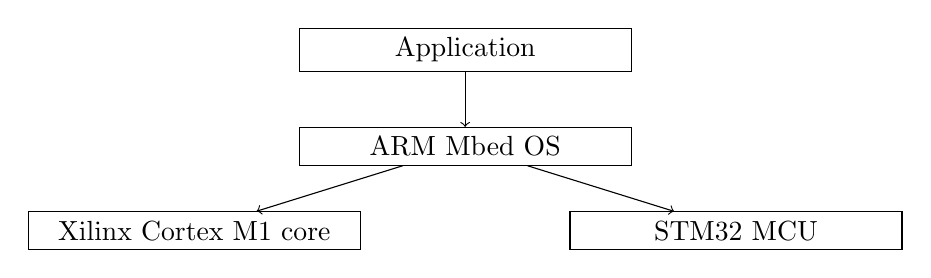
\begin{tikzpicture}[
    node distance = 7mm and 12mm,% for distance between nodes
       box/.style = {draw, minimum width=12em}% nodes style
    ]
    \node (app) [box] {Application};
    \node (mbed) [box, below=of app.south] {ARM Mbed OS};
    \node (ph) [below=of mbed.south] {};
    \node (xilinx) [box, left=of ph.west] {Xilinx Cortex M1 core};
    \node (stm) [box, right=of ph.east] {STM32 MCU};
    \draw[->] (app) edge (mbed);
    \draw[->] (mbed) edge (xilinx);
    \draw[->] (mbed) edge (stm);
\end{tikzpicture}
\caption{Software structure.}\label{fig:mbed}
\end{figure}


\chapter{Communication Protocol}

This section describes the communication protocol used for command and data exchange between bus participants. Further, the bus monitor module, which is part of the \gls{FBU} is explained.

\section{Protocol}

In our approach a simple master-slave protocol was defined to enable communication between the master (\gls{ECU}, \gls{FBU}) and the slaves (\gls{THS}, \gls{MCU}, \gls{FBU}).
The protocol consists of command and data packets, each of them contains just one byte.
No error protection measures were taken into account.
Each bus participant needs a unique address. Since this design just contains three control units, two bits as address field are sufficient. Figure \ref{fig:ControlPacket} shows the composition of a control packet.

\begin{figure}[h!]
    \centering
    \includegraphics[width=\textwidth]{figures/ControlPacket.pdf}
    \caption{Composition of a control packet}\label{fig:ControlPacket}
\end{figure}

A control packet is indicated by two leading zeroes. Followed by source address (2 bits) and destination address (2 bits).

\section{Bus monitor}

How is it set up?

Made assumptions?

Document used / invented protocol.


\section{Partial Reconfiguration}
What is partially reconfigured - Cortex, uart, IIC.

Why not use AXI?

\subsection{Integration Overview}
\cite{xilinx_vivado_2018-1}, \cite{xilinx_vivado_2018}
Usage of ICAP.

How is the Zynq still used - Loading images and binary blobs from sd card into DDR.

\subsection{Packaged IP}
Why is the PR IP Packaged, how was it done? \cite{noauthor_ug1118-vivado-creating-packaging-custom-ip.pdf_nodate}

%\section{Organization}

\subsection{Assigned Sub-Tasks}
 \subsubsection{Cortex M1} 
 Evaluation of the provided Cortex-M1 from ARM and adaption of the provided toolchain to our needs. 

 Creation of a working stand-alone example, creation and integration of working IP-Packages for the Cortex-M1
 \subsubsection{Partial Reconfiguration} 
 \subsubsection{Bus Design}
 \subsubsection{Hardware}   
\subsection{Estimated Contribution}
Contribution to the project was roughly the same for each group member.
    \begin{table}
        \centering
\begin{tabular}{ l | c c c c c}
 Task & Hirtenlehner & Schieber & Schober & Schorn\\ 
 \hline
Cortex M1       & X & X & X & \\
Partial Reconf. & X & X & & \\
Bus Design      & & & & X\\
Hardware        & X & & & X\\
Mbed OS         & X & & & X\\
\end{tabular}
\caption{Distribution of tasks within the group}
\end{table}
\chapter{Results}
Results would usually encompass benchmarks on the following things:
\begin{itemize}
    \item Time to reconfigure
    \item Time to fault detection
    \item Time to fault mitigation
    \item Fault Mitigation success rate
\end{itemize}
Time constraints and a hardware set-up that is not yet ready to be benchmarked extensively (e.g. benchmarking infrastructure missing, stability problems) only allow us to give us a basic overview over the used resources.

\subsection{Resource Usage}
The design currently uses around 11\% of the Zynqs available hardware resources, a detailed key is given in table \ref{tbl:resourceUtilization}.
Most of the resource usage can be accounted to the \gls{RP} as it contains the Cortex-M1 with its high demand for BRAM elements.
This demand is easily visible in the implemented design (figure \ref{fig:implementation}).
\begin{table}
    \centering
\begin{tabular}{ l | l l l} 
Type    &Used&Available&Percent [\%] used\\
\hline
LUT	    &4827   &53200	&9.07\\
LUTRAM	&289    &17400	&1.66\\
FF	    &4832	&106400	&4.54\\
BRAM    &16	    &140	&    11.42\\
DSP	    &3	    &220	 &   1.36\\
IO	    &25	    &200	 &   12.50\\
BUFG	&3	    &32	    &9.37\\
MMCM	&1	     &4	    &25.00\\
\hline
\end{tabular}
\caption{Resource utilization, post-implemntation}
\end{table}\label{tbl:resourceUtilization}

\begin{figure}[h!]
    \centering
    \includegraphics[width=0.75\textwidth]{figures/implementation.pdf}
    \caption{Implemented design, \gls{RP} in the right bottom corner.}\label{fig:implementation}
\end{figure}

\subsection{Open Issues}
\begin{itemize}
    \item Partial reconfiguration fails for one bitstream and results in a voltage drop, see section \ref{sec:voltageDrop}.
    \item Partial Reconfiguration Controller only works with a manual reset after start-up
\end{itemize}
\subsection{Instability of Voltage Supply during \gls{PR}}\label{sec:voltageDrop}
During the process of partial reconfiguration for the Cortex M1 engine module a voltage drop (2V) occurs on the hardware setup.
\begin{figure}[h!]
    \centering
    \includegraphics[width=0.75\textwidth]{figures/voltageDropPR.jpg}
    \caption{}\label{fig:voltageDropPR}
\end{figure}

\chapter{Conclusion}
This work has explored the possibility of using partial reconfiguration in \glspl{FPGA} to provide efficient redundancy in an automotive system.
Instead of providing a redundant hardware entity for every critical module, one single \gls{FPGA} provides dynamic redundancy for each of these modules.
To avoid over-commitment with regards to resource usage (space and power) partial reconfiguration is used.
By using the newly available Cortex M1 IPs, a streamlined software development process is possible. 
The same software can be executed on the cores in the \gls{FPGA} as well as on the actual hardware with minimal adaptions in the build-process.
This reduces the amount of testing and tool-chain adaptions that need to be performed.
We demonstrated these concepts on the Zynq-7000 and with three Cortex M1 \glspl{CPU} that were connected with a bus.

\section{Future Work}
Based on this work a more heterogeneous set of critical hardware could be provided with redundancy. 
A good first step would be to include the Cortex M3 CPU that couldn't be included in this project due to time constraints.
The bus monitor could be extended with a more sophisticated fault detection algorithm, which could also mean to employ a more sophisticated bus protocol.
Measurements with regards to the system performance (e.g. time to reconfigure, time to detect fault, time to mitigate fault, power usage ...) should be considered also.  

\bibliographystyle{IEEEtran}
\bibliography{IEEEabrv,SoCLabor}

\end{document}

